\documentclass[12pt]{article}

\usepackage{sbc-template}
\usepackage{graphicx,url}
\usepackage[utf8]{inputenc}
\usepackage[brazil]{babel}
\usepackage{listings}
\usepackage{xcolor}

\lstset{
    basicstyle=\ttfamily\footnotesize,
    breaklines=true,
    frame=single,
    showstringspaces=false,
    columns=fullflexible,
    keywordstyle=\bfseries,
    commentstyle=\itshape\color{gray!70!black}
}

\sloppy

\title{Trabalho Prático 1 --- Implementação de um Controlador de \emph{Cache}
em SystemVerilog}

    %\author{Antônio Drumond Cota de Sousa{\thanks{Antonio Sousa is an undergraduate student in Computer Science at PUC Minas.}}, Henrique Cota de Freitas{\thanks{The authors thank FIP PUC Minas for the support provided in carrying out this scientific initiation.}}}
    \author{Antônio D. C Sousa, Davi F. Puddo, Gabriel V. B. Silva,\\ Mateus H. M. Diniz, Raquel P. Motta}

\address{Graduação em Ciência da Computação\\
Instituto de Ciências Exatas e Tecnologia, PUC Minas\\
Caixa Postal, 1.686 – Belo Horizonte – MG – Brazil\\
   Minas Gerais -- MG -- Brasil
  \email{\ \{adcsousa,davi.puddo,gabriel.silva.1524976\}@sga.pucminas.br}
  \email{\ \{mateus.diniz.880541,raquel.motta\}@sga.pucminas.br}
}

\begin{document}

\maketitle

\begin{resumo}
Este relatório descreve a implementação de um controlador de \emph{cache}
em SystemVerilog, baseado no Capítulo~5, Seção~5.12 do livro
\emph{Computer Organization and Design: The Hardware/Software Interface
--- RISC-V Edition}, de Patterson e Hennessy. O projeto consiste em uma
\emph{cache} de mapeamento direto, com 1024 linhas de 128 \emph{bits},
política \emph{write-back} com \emph{write-allocate}, descrita como uma
máquina de estados finitos. São discutidas as decisões de projeto, as
dificuldades encontradas, a estrutura do \emph{testbench} usado para validação
funcional e o papel das ferramentas de IA no processo.
\end{resumo}

\begin{abstract}
This report describes the implementation of a cache controller in
SystemVerilog, based on Chapter~5, Section~5.12 of \emph{Computer
Organization and Design: The Hardware/Software Interface --- RISC-V
Edition} by Patterson and Hennessy. The design is a direct-mapped cache
with 1024 lines of 128~bits, using a write-back / write-allocate policy
and structured as a finite-state machine. We discuss design decisions,
issues encountered,
the structure of the testbench used for functional validation, and the
role of AI tools throughout the process.
\end{abstract}

\section{Introdução}

\emph{Caches} reduzem a diferença de latência entre CPU e memória
principal explorando localidade temporal e espacial. Este trabalho
implementa o controlador de \emph{cache} descrito na Seção~5.12
de \cite{patterson:2021}, em SystemVerilog. Trata-se de uma
\emph{cache} \emph{blocking}, de mapeamento direto, com 1024 blocos
de 128 \emph{bits}, política \emph{write-back} com
\emph{write-allocate} e um bit \texttt{valid} e um bit
\texttt{dirty} por linha. A Figura~\ref{fig:diagrama} reproduz o
diagrama em blocos do livro, com os nomes dos sinais usados na
descrição em SystemVerilog, que serviu de referência principal para a implementação.

A proposta envolveu usar os exemplos de código fornecidos no livro e seu material complementar como base para codificar um simulador compilável e funcional. 

\begin{figure}[ht]
\centering
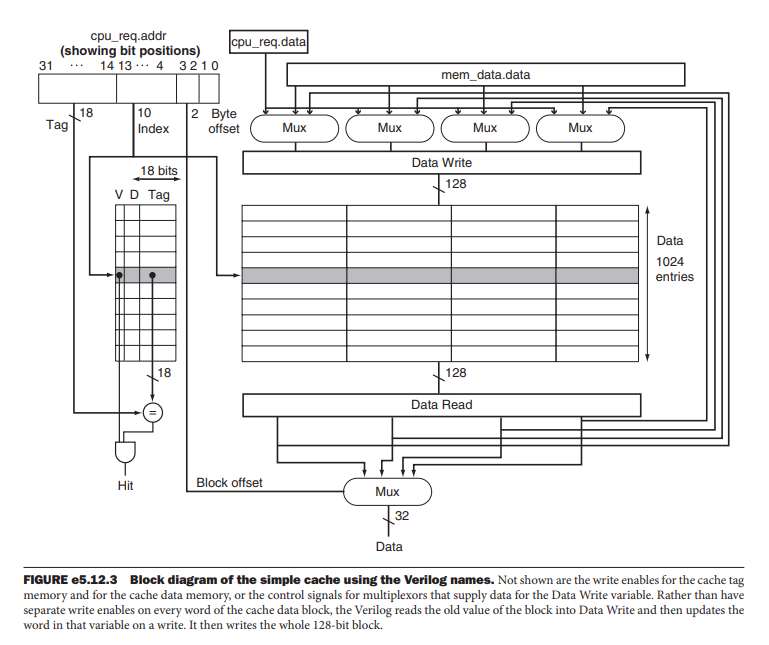
\includegraphics[width=.85\textwidth]{fig_e5123_livro.png}
\caption{Diagrama em blocos da \emph{cache} usando os nomes do
SystemVerilog, conforme Figura~e5.12.3 do livro~\cite{patterson:2021}.}
\label{fig:diagrama}
\end{figure}

\subsection{Visão geral da arquitetura}

O projeto está em \texttt{src/cache\_def.sv} e contém três módulos:
\texttt{dm\_cache\_data} (memória de dados, 1024 linhas de 128
\emph{bits}), \texttt{dm\_cache\_tag} (memória de \emph{tags},
mesma profundidade, com \texttt{valid}, \texttt{dirty} e o vetor de
\emph{tag}) e \texttt{dm\_cache\_fsm} (contém toda a lógica de
controle). As memórias
têm escrita síncrona com \emph{write enable} e leitura combinacional,
exatamente como em \cite{patterson:2021}.

O endereço de 32 \emph{bits} é decomposto em \emph{tag}
(\texttt{addr[31:12]}), índice (\texttt{addr[11:2]}) e seletor de
palavra dentro da linha (\texttt{addr[1:0]}), de modo a indexar 4
palavras de 32 \emph{bits} por linha. Os bits da \emph{tag} são
referenciados pelos parâmetros \texttt{TAGMSB} e \texttt{TAGLSB}.

\begin{center}
\begin{tabular}{|c|c|c|}
\hline
\scriptsize 31 \hfill 12 & \scriptsize 11 \hfill 2 & \scriptsize 1 \hfill 0 \\
\hline
\textbf{Tag} & \textbf{Índice da linha} & \textbf{Byte Offset} \\
20 bits & 10 bits & 2 bits \\
\hline
\end{tabular}
\end{center}

A CPU e a memória
principal não fazem parte do controlador propriamente dito: são
simuladas a partir do \emph{testbench}. Para a CPU, o arquivo de \emph{testbench} simplesmente envia requisições de leitura/escrita
\emph{hard-coded}. Para a memória, foi utilizado um arranjo associativo que funciona de modo semelhante a um dicionário ou tabela hash, e gera dados aleatórios para popular endereços acessados pela primeira vez.

\section{Desenvolvimento}

O código apresentado no livro mistura SystemVerilog com convenções
tipográficas próprias e contém pequenas incorreções (espaçamento
ausente entre tipo e identificador, uso de aspas invertidas no lugar
de apóstrofo em literais \texttt{'0}, falta de \texttt{begin/end} em
alguns ramos do \texttt{case}). A primeira etapa consistiu em
transcrever as linhas para um único arquivo
\texttt{.sv} e ajustar essas construções até obter compilação
limpa, garantindo também que todos os sinais do bloco
\texttt{always\_comb} fossem inicializados com valores
\emph{default}, evitando inferência de \emph{latches}.

\subsection{Máquina de estados}
Após a adaptação inicial do código, o próximo passo foi estudar e mapear o comportamento da FSM (Máquina de Estados Finitos) que rege o funcionamento da cache, que contém quatro
estados: \texttt{idle}, \texttt{compare\_tag}, \texttt{allocate} e
\texttt{write\_back}. O diagrama que produzimos está ilustrado na Figura~\ref{fig:fsm}.

\begin{figure}[ht]
\centering
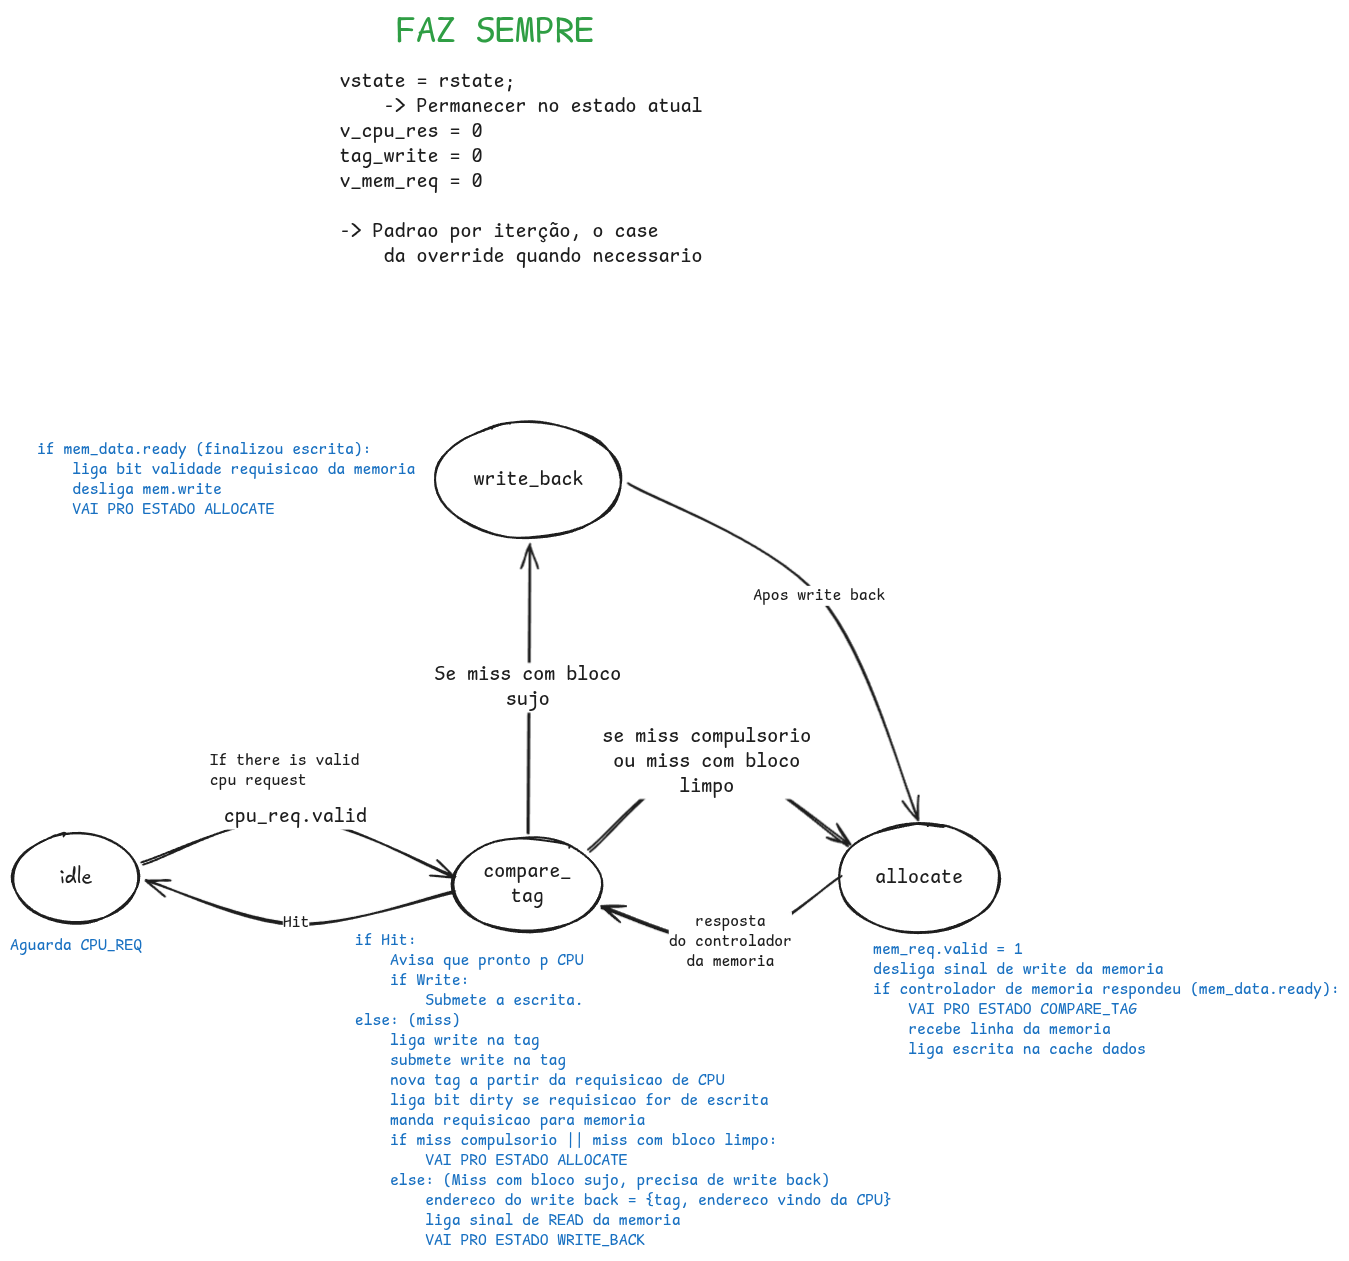
\includegraphics[width=.95\textwidth]{maquinaEstadosAntonio.png}
\caption{Máquina de estados do controlador de \emph{cache}, com
transições, condições e ações associadas a cada estado.}
\label{fig:fsm}
\end{figure}

No estado \texttt{idle}, a FSM apenas espera por uma requisição da CPU: quando \texttt{cpu\_req.valid = 1}, ocorre a transição para \texttt{compare\_tag}. Nesse segundo estado, comparam-se a \emph{tag} lida da memória de \emph{tags} com a \emph{tag} do endereço pedido, levando em conta também o bit \texttt{valid} da entrada. Se houver \emph{hit}, a transação se resolve em um único ciclo --- \texttt{cpu\_res.ready = 1} e a FSM volta direto para \texttt{idle}. No caso particular de um \emph{write hit}, a linha correspondente ainda é marcada como \texttt{dirty} antes do retorno. 

Se houver \emph{miss}, dois caminhos são possíveis: (1) quando o bloco atualmente alocado naquele índice é \emph{clean} (dirty bit desativado indica que não modificamos os dados da cache e, portanto, não há necessidade de copiá-los para a memória) ou quando o bit \texttt{valid} está em zero (caracterizando um \emph{miss} compulsório, isto é, os dados naquele espaço são descartáveis). Nesses casos, parte-se direto para \texttt{allocate}. (2) quando o bloco for \emph{dirty}. É preciso primeiro escrevê-lo de volta na memória principal, e por isso a FSM passa por \texttt{write\_back} antes de chegar em \texttt{allocate}.

No estado \texttt{allocate}, mantém-se uma requisição de leitura à memória principal até que ela responda com \texttt{mem\_data.ready}; quando isso acontece, a linha da \emph{cache} é atualizada e a FSM volta para \texttt{compare\_tag}, e dessa vez o acesso necessariamente vai dar \emph{hit}, porque a linha correta acabou de ser carregada. Já em \texttt{write\_back} a lógica é mais simples: ficamos esperando o \emph{ack} da memória e, assim que ele chega, submetemos imediatamente a requisição de leitura nova (para a linha que vai substituir a antiga) e seguimos para \texttt{allocate}.

\subsection{Comunicação entre CPU, cache e memória}

O controlador conversa em duas interfaces:

\begin{itemize}
    \item Com a CPU, recebe \texttt{CPURequest} (endereço, dado,
    tipo de operação \texttt{rw} e um bit \texttt{valid}) e devolve
    \texttt{CPUResult} (dado lido e um bit \texttt{ready}).
    \item Com a memória, envia \texttt{MemRequest} (endereço, linha
    de 128 \emph{bits}, \texttt{rw} e \texttt{valid}) e recebe
    \texttt{MemData} (linha lida e \texttt{ready}).
\end{itemize}

Em ambas, o bit \texttt{valid} cumpre o
papel de \emph{request strobe} (um strobe é um sinal de controle dedicado usado para sincronizar a transferência de dados entre dois componentes de hardware): do lado da CPU, indica que há um
acesso a ser tratado; do lado do controlador, indica à memória que
uma requisição está sendo submetida naquele ciclo. 

A memória só
toma o trabalho de responder quando \texttt{req.valid} estiver em 1. No estado \texttt{compare\_tag}, por exemplo, o
\texttt{v\_mem\_req.valid} só é levantado \emph{quando o caminho
de \emph{miss} é percorrido}. Nos demais casos ele é deixado em
zero pelo \emph{default} do início do bloco combinacional. Isso foi
uma dúvida do grupo, e o prompt usado para investigá-la está na seção sobre uso de IA. 

Por fim, o bit \texttt{ready} 
sinaliza ao controlador que a memória já terminou de processar a
requisição. Como
\texttt{v\_mem\_req.valid} é zerado por \emph{default} no início do
\texttt{always\_comb}, ele só sobe nos ramos da FSM em que de fato
ocorre acesso à memória (caminho de \emph{miss}), evitando
requisições espúrias.

Do ponto de vista da modelagem, essas interfaces
constituem uma abstração das conexões físicas entre módulos. Em uma
implementação em \emph{hardware}, a comunicação entre CPU, cache e
memória se daria por meio de barramentos --- conjuntos de sinais
elétricos roteados entre os blocos. Na descrição em SystemVerilog,
esses barramentos são representados por estruturas tipadas
(\texttt{CPURequest}, \texttt{CPUResult}, \texttt{MemRequest} e
\texttt{MemData}) cujos campos agregam todos os sinais de uma
direção do barramento em um único objeto, manipulado por nome no
corpo dos módulos. As variáveis intermediárias \texttt{v\_mem\_req}
e \texttt{v\_cpu\_res}, atualizadas no bloco \texttt{always\_comb} e
amarradas às portas de saída por meio de \texttt{assign}, exercem
o papel de \emph{buffers} de interface entre o estado interno da
FSM e os módulos vizinhos, garantindo que cada ciclo apresente um
valor bem definido em cada porta. A Figura~\ref{fig:fsm} ilustra essa abstração.

\begin{figure}[ht]
\centering
\includegraphics[width=.5\textwidth]{comunicacaoCPUCacheMem.png}
\caption{Comunicação entre módulos. As caixas vermelhas
representam as estruturas tipadas
que substituem os barramentos físicos do hardware.}
\label{fig:comunication}
\end{figure}

\subsection{Dificuldades com a memória simulada}

A descrição original da memória simulada usava um arranjo associativo declarado como \texttt{bit [127:0] mem[*]}. Em SystemVerilog, esse \texttt{[*]} indica um \emph{wildcard associative array}, em que a chave é qualquer valor inteiro.

O problema é que essa construção não é suportada de forma satisfatória pelo Verilator (a ferramenta usada neste trabalho), e algumas operações sobre o arranjo não funcionavam como o esperado, especialmente a operação de gravar dados no arranjo. O resultado era que a memória retornava 0 em todas as operações de leitura. Foi um dos pontos em que perdemos mais tempo de \emph{debug}, porque a FSM parecia estar funcionando corretamente, mas todas as operações de leitura na memória tinham 0 como resultado, mesmo após gravar dados no mesmo endereço, quando na verdade o problema estava do outro lado da interface, na memória simulada.

A solução foi trocar o \texttt{[*]} por uma chave de tipo explícito, com largura coerente com o endereçamento que estamos usando:

\begin{lstlisting}[language=Verilog]
bit [127:0] mem[reg[29:0]];
\end{lstlisting}

A escolha do uso de 30 bits e não 32 para endereçar a memória foi feita para invalidar endereços muito altos no ponto de vista da cache de forma a explorar o comportamento da cache e memória simuladas quando acesso for feito a endereços extremos.

\subsection{Outros desafios e decisões de projeto}

A nível arquitetural, seguimos a proposta do livro: mapeamento direto com 1024 linhas de 128
\emph{bits}; política \emph{write-back} (a linha só é gravada na
memória ao ser substituída, controlada pelo bit \texttt{dirty})
combinada com \emph{write-allocate} (em \emph{write miss} o bloco
é carregado antes da escrita); FSM Moore, com estado registrado e
saídas calculadas em um único \texttt{always\_comb}; e interfaces
com \texttt{valid}/\texttt{ready} como \emph{handshake}.

No nível do código, além da questão da memória simulada, outros pontos exigiram decisão própria. O
primeiro foi de \emph{legibilidade}: os \texttt{typedef}s originais
(\texttt{cache\_tag\_type}, \texttt{cpu\_req\_type}, etc.) foram
preservados por consistência com o livro, mas receberam
\emph{aliases} em \emph{PascalCase} usados nas declarações de
portas e sinais (\texttt{CPURequest cpu\_req} lê mais
naturalmente do que \texttt{cpu\_req\_type cpu\_req}). A
\emph{struct} de \emph{tag} mantém os campos nomeados
(\texttt{valid}, \texttt{dirty}, \texttt{tag}), permitindo acesso
por nome no corpo da FSM.

O segundo foi a \emph{parametrização} de \texttt{TAGMSB} e
\texttt{TAGLSB}. No livro, ambos são introduzidos como
\texttt{parameter int} com valores 31 e 14. Mantivemos a
parametrização, mas com \texttt{TAGLSB = 12}, refletindo a opção
por usar \texttt{addr[1:0]} como seletor de palavra dentro da linha
(em vez de \texttt{addr[3:2]} como no livro, que pressupõe
endereçamento \emph{byte-aligned}). Centralizar esses valores no
pacote \texttt{cache\_def}, em vez de espalhá-los como literais
pelo RTL, isola a geometria da \emph{cache} em um único ponto.

\section{Testes de validação}
\subsection{Estrutura do \emph{testbench}}

O ambiente de simulação foi desenvolvido em um único arquivo contendo 
dois módulos principais: \emph{sim\_mem}, responsável por emular o comportamento 
e os atrasos da memória principal, e \emph{test\_main}, que atua como o \emph{testbench} 
propriamente dito. O módulo principal instancia a FSM da cache, gerencia o 
clock e aplica um pulso de reset (\emph{rst}), colocando o controlador em seu estado inicial. Vale ressaltar que, devido à tipagem bit do SystemVerilog, todos os arrays de dados e tags são inicializados com 0 por padrão. Ademais, a sequência de instruções
básicas necessárias para leitura e escrita foram encapsuladas em \emph{read}
e \emph{write} respectivamente, além de padronizar as estruturas de validação de testes com
exibição visual, para facilitar a compreensão e implementação.

\begin{lstlisting}[language=Verilog]
        task read(input bit[31:0] address);
            iu_req.rw = '0;
            iu_req.addr = address;
            iu_req.valid = '1;
            wait(iu_res.ready == '1);
        endtask

        task write(input bit[31:0] address, input bit[31:0] data);
            iu_req.rw = '1;
            iu_req.addr = address;
            iu_req.data = data;
            iu_req.valid = '1;
            wait(iu_res.ready == '1);
        endtask
         `define mksection(number, title) \
            $display("\033[35m%s\033[0m: \033[36m%s\033[0m", number, title);

        `define check_test(name, lhs, rhs, op) \
            if (lhs op rhs) begin \
                $display("\t\033[34mtest [%s]\033[0m: \033[32mok\033[0m", name); \
            end else begin \
                $display("\t\033[34mtest [%s]\033[0m: \033[31mfailed\033[0m", name); \
            end \
            $display("\t\tCondition: \033[36m%s\033[0m (\033[33m%h\033[0m) \033[35m%s\033[0m \033[36m%s\033[0m (\033[33m%h\033[0m)", `"lhs`", lhs, `"op`", `"rhs`", rhs); \
            iu_req.valid = 0; \
            #5;

\end{lstlisting}

\subsection{Etapas de teste}

O testes foram divididos em cinco etapas: i) Testes de Leitura (Read Path); 
ii) Teste de Escrita (Write Path); iii) Testes de Substituição; iv) Testes de Consistência 
e v) Testes de Casos Limite. Que por sua vez foram subdivididos de acordo com as
etapas necessárias para o objetivo.

\subsubsection{Leitura}

Nesse momento, o objetivo é validar o funcionamento correto das operações de leitura, nos casos de hit, com os dados requeridos já devidamente armazenados em cache, e com necessidade de acesso a memória principal, verificando posteriormente a atualização dos bits de controle: \emph{tag} e \emph{valid}.

Em relação ao hit, é necessário implementar duas leituras no mesmo endereço, onde a primeira resultaria em miss compulsório, tornando necessária a busca dos dados na memória principal como alocação inicial. Dessa forma, possibilita-se que a segunda realize o hit efetivo, aguardando um intervalo de tempo simulado entre ambas, validando por meio da análise do status da última requisição.

\begin{lstlisting}[language=Verilog]
            `mksection("7.1.1", "Access with cache hit");
            read(0);
            iu_req.valid = 0;
            #5;
            read(0);
            prev_hit = iu_res.hit;
            `check_test("checking hit on read", prev_hit, 1, ==);
\end{lstlisting}

Para garantir a não ocorrência de um falso hit (quando a cache ignora a mudança de tag), simulou-se um acesso à memória principal forçando uma substituição de bloco. Foram realizadas operações de escrita nos endereços 0x00000000 e 0x00001000, que, por compartilharem os mesmos bits de índice, mapeiam para a mesma linha da cache. Posteriormente, eles são acessados para leitura na mesma sequência, momento em que são realizadas duas verificações: se a segunda leitura acarretou em um miss e se os dados da primeira leitura diferem da segunda.

\begin{lstlisting}[language=Verilog]
            `mksection("7.1.2", "Access with cache hit followed by memory load");
            write('h00000000, 'hF00DCAFE);
            write('h00001000, 'hCAFEBABE);
            read('h00000000);
            prev_data = iu_res.data; 
            #5;
            read('h00001000);
            `check_test(
                "checking miss data change on read", 
                prev_data, iu_res.data, !=
            );
            `check_test(
                "checking miss on read", 
                iu_res.hit, 0, ==
            );
\end{lstlisting}

A fim de validar os bits de controle \emph{tag} e \emph{valid}, foram realizadas duas leituras no endereço 0xCAFFE000 a primeira deve ocasionar um miss com  \emph{iu\_res.line\_tag.valid = 0} e assim trazer os dados com a respectiva tag 0xCAFFE da memória, uma segunda leitura ao mesmo endereço visa constatar que o bit de validade agora indica que o endereço desejado já esta presente na cache.

\begin{lstlisting}[language=Verilog]
                `mksection("7.1.3", "Tag & valid bit values");
            read('hCAFFE000);
            `check_test(
                "checking tag value after allocation",
                iu_res.line_tag.tag, 'hCAFFE, ==
            );
            `check_test(
                "checking valid bit value after allocation",
                iu_res.line_tag.valid, '0, ==
            );
            read('hCAFFE000);
            `check_test(
                "checking valid bit value on hit",
                iu_res.line_tag.valid, '1, ==
            );
\end{lstlisting}

\subsubsection{Escrita}

Para a avaliação do caminho de dados de escrita, foram simuladas três situações: escrita com \emph{hit}, escrita com \emph{miss} e validação do bit de controle de modificação (\emph{dirty}) referente à política de escrita. A primeira validação foi implementada realizando operações de leitura e escrita de forma subsequente sobre o mesmo endereço. A leitura inicial atua como um \emph{miss} compulsório, garantindo que o bloco seja alocado na \emph{cache}. Dessa forma, a operação de escrita logo em seguida resulta obrigatoriamente em um \emph{hit}. Por fim, uma nova leitura é realizada para constatar se os dados foram devidamente atualizados e armazenados na \emph{cache} interna.
\begin{lstlisting}[language=Verilog]
            `mksection("7.2.1", "Write with hit");
            read('h00002000);
            `check_test("allocating block for write", iu_res.hit, 0, ==);
            write('h00002000, 'hDEADBEEF);
            `check_test("checking write hit", iu_res.hit, 1, ==);
            read('h00002000);
            `check_test("checking data written on hit", iu_res.data, 'hDEADBEEF, ==);
\end{lstlisting}

Posteriormente, para o teste de escrita com \emph{miss} e para a comprovação da política de \emph{Write-Allocate} (alocação na escrita), a \emph{cache} recebeu uma instrução de escrita direta em um endereço arbitrário que ainda não havia sido acessado. Espera-se que essa operação acarrete um \emph{miss}, forçando o controlador a buscar o bloco na memória principal antes de aplicar a modificação. O sucesso da alocação e da escrita é validado por uma leitura subsequente, submetendo o endereço à mesma análise anterior para atestar se o dado retornado é exatamente o valor recém-escrito.

\begin{lstlisting}[language=Verilog]
            `mksection("7.2.2", "Write with miss");
            write('h00003000, 'hBEEFCAFE);
            `check_test("checking write miss", iu_res.hit, 0, ==);
            read('h00003000);
            `check_test("checking data written on miss", iu_res.data, 'hBEEFCAFE, ==);
\end{lstlisting}

A seguir, a simulação foi direcionada à validação da política de \emph{Write-Back} (escrita postergada). Para isso, realizou-se a escrita em um novo endereço arbitrário, seguida imediatamente por uma leitura de inspeção. O objetivo dessa leitura posterior é revelar o estado dos metadados da \emph{cache}, exigindo que o controlador tenha ativado corretamente o bit \emph{dirty} (\emph{iu\_res.line\_tag.dirty == 1}), sinalizando que o bloco sofreu modificação local e está inconsistente em relação à memória principal.

\begin{lstlisting}[language=Verilog]
            `mksection("7.2.3", "Write policy");
            write('h00004000, 'h12345678);
            `check_test("allocating for policy check", iu_res.hit, 0, ==);
            read('h00004000);
            `check_test("checking dirty bit on write", iu_res.line_tag.dirty, 1, ==);
\end{lstlisting}

\subsubsection{Substituição}
A simulação para as políticas de substituição foi realizada visando avaliar tanto a substituição simples (de blocos não modificados) quanto a substituição de dados em estado \emph{dirty}, que demandam a utilização do mecanismo de \emph{write-back}. A princípio, foram realizadas duas leituras em endereços diferentes que mapeiam para o mesmo índice na \emph{cache}, provocando uma substituição de bloco. Uma terceira leitura, realizada novamente sobre o primeiro endereço, teve como objetivo verificar se a evicção ocorreu como o esperado. A análise do bit \emph{hit} atesta que todas as três operações levaram a um \emph{miss}, comprovando o correto funcionamento do mapeamento direto.

\begin{lstlisting}[language=Verilog]
            `mksection("7.3.1", "Cache fill & block substitution");
            read('h00005000);
            `check_test("checking fill miss", iu_res.hit, 0, ==);
            read('h00006000);
            `check_test("checking substitution miss", iu_res.hit, 0, ==);
            `mksection("7.3.2", "Cache substitution policy");
            read('h00005000);
            prev_hit = iu_res.hit;
            `check_test("checking direct mapped eviction", iu_res.hit, 0, ==);
\end{lstlisting}

Para validar a funcionalidade de \emph{write\_back}, simulou-se a criação de um bloco \emph{dirty} através de uma operação de escrita no endereço 0x00007000. Posteriormente, uma leitura no endereço 0x00008000, que mapeia para o mesmo índice da escrita anterior, forçou uma nova substituição. Devido ao estado sujo da linha, tornou-se necessária a reescrita prévia do bloco antigo na memória principal antes da alocação do novo. Por fim, para confirmar a correta transição de estados do controlador, observou-se o sinal \emph{iu\_res.write\_back}, cujo valor em nível lógico alto atesta a aplicação rigorosa da política.

\begin{lstlisting}[language=Verilog]
            `mksection("7.3.3", "Write-back");
            write('h00007000, 'hAABBCCDD);
            `check_test("write allocating 7000", iu_res.hit, 0, ==);
            read('h00008000);
            `check_test("checking write-back occurred", iu_res.write_back, 1, ==);
\end{lstlisting}

\subsubsection{Consistência}

Para avaliar a consistência do controlador, foram implementadas três simulações distintas. A primeira verifica a coerência de dados, realizando a escrita em um endereço seguida imediatamente por uma leitura, a fim de validar se os dados recém-modificados foram efetivamente armazenados e disponibilizados. A segunda analisa o comportamento da máquina de estados diante de acessos de leitura sequenciais a um mesmo endereço, observando a ocorrência de um \emph{miss} compulsório inicial seguido de \emph{hits} ininterruptos. Por fim, a terceira simulação aborda cenários de conflito, alternando acessos de leitura a diferentes endereços que mapeiam para o mesmo índice na \emph{cache}. A validação ocorre através da análise do bit de \emph{hit}, confirmando que cada requisição alternada resulta em um novo \emph{miss} devido à evicção contínua dos blocos.

\begin{lstlisting}[language=Verilog]
            `mksection("7.4.1", "Data coherence");
            write('h00009000, 'h99999999);
            `check_test("write allocating 9000", iu_res.hit, 0, ==);
            read('h00009000);
            `check_test("checking data coherence read after write", iu_res.data, 'h99999999, ==);
            `mksection("7.4.2", "Repeated address access");
            read('h0000A000);
            `check_test("first read miss", iu_res.hit, 0, ==);
            read('h0000A000);
            `check_test("checking hit on repeated access", iu_res.hit, 1, ==);
            read('h0000A000);
            `check_test("checking hit on 3rd access", iu_res.hit, 1, ==);
            `mksection("7.4.3", "Conflicts");
            read('h0000B000);
            `check_test("first read B000", iu_res.hit, 0, ==);
            read('h0000C000);
            `check_test("first read C000", iu_res.hit, 0, ==);
            read('h0000B000);
            `check_test("checking conflict miss", iu_res.hit, 0, ==);
\end{lstlisting}

\subsubsection{Casos limite}

Para finalizar a validação do controlador, a última etapa de testes avalia o comportamento da \emph{cache} em situações extremas e verifica a integridade de seu estado inicial. A primeira simulação analisa o acesso a endereços nos limites absolutos do barramento de 32 bits (como 0xFFFFFFFF e 0xFFFFFFF0), atestando que o roteamento de bits e o alinhamento de blocos operam corretamente sem causar falhas ou \emph{overflows} nos registradores. A segunda abordagem foca na inicialização tardia, realizando a leitura de um endereço arbitrário virgem para garantir que o estado padrão da \emph{cache} (linhas invalidadas) não sofreu corrupção durante o estresse das dezenas de operações e evicções anteriores. Por fim, a terceira simulação expande essa verificação ao executar leituras consecutivas em múltiplos blocos intocados, assegurando a robustez do isolamento da \emph{cache} e a ausência de vazamento de metadados entre linhas vizinhas. Em todos os cenários, a validação é confirmada pela análise do bit de \emph{hit}, exigindo rigorosamente que todas as requisições resultem em \emph{misses}.

\begin{lstlisting}[language=Verilog]
            `mksection("7.5.1", "Edge case access");
            read('hFFFFFFFF);
            `check_test("checking edge case miss FFFFFFFF", iu_res.hit, 0, ==);
            read('hFFFFFFF0);
            `check_test("checking edge case FFFFFFF0", iu_res.hit, 0, ==);
            `mksection("7.5.2", "Cache initialization");
            read('h0000D000);
            `check_test("checking initialization miss on untouched address", iu_res.hit, 0, ==);
            `mksection("7.5.3", "Fully invalid cache behavior");
            read('h0000E000);
            `check_test("checking miss E000", iu_res.hit, 0, ==);
            read('h0000F000);
            `check_test("checking miss F000", iu_res.hit, 0, ==);
\end{lstlisting}

\subsection{Resultados}
Os resultados obtidos na simulação foram plenamente coerentes com o comportamento esperado em cada bateria de testes. O registro de execução atesta o sucesso da implementação do controlador de \emph{cache}, validando a eficácia de suas políticas de alocação e substituição, bem como a sua estabilidade diante de casos extremos e cenários de estresse que poderiam induzir falhas no sistema. Conforme o relatório de saída gerado pelo simulador Verilator, todas as asserções lógicas foram cumpridas sem apresentar erros, finalizando a verificação com êxito.

\begin{lstlisting}
7.1.1: Access with cache hit
        test [checking hit on read]: ok
                Condition: prev_hit (1) == 1 (00000001)
7.1.2: Access with cache hit followed by memory load
        test [checking miss data change on read]: ok
                Condition: prev_data (409b89cf) != iu_res.data (3dfa6bf3)
        test [checking miss on read]: ok
                Condition: iu_res.hit (0) == 0 (00000000)
7.1.3: Tag & valid bit values
        test [checking tag value after allocation]: ok
                Condition: iu_res.line_tag.tag (caffe) == 'hCAFFE (000caffe)
        test [checking valid bit value after allocation]: ok
                Condition: iu_res.line_tag.valid (0) == '0 (0)
        test [checking valid bit value on hit]: ok
                Condition: iu_res.line_tag.valid (1) == '1 (1)
7.2.1: Write with hit
        test [allocating block for write]: ok
                Condition: iu_res.hit (0) == 0 (00000000)
        test [checking write hit]: ok
                Condition: iu_res.hit (1) == 1 (00000001)
        test [checking data written on hit]: ok
                Condition: iu_res.data (deadbeef) == 'hDEADBEEF (deadbeef)
7.2.2: Write with miss
        test [checking write miss]: ok
                Condition: iu_res.hit (0) == 0 (00000000)
        test [checking data written on miss]: ok
                Condition: iu_res.data (beefcafe) == 'hBEEFCAFE (beefcafe)
7.2.3: Write policy
        test [allocating for policy check]: ok
                Condition: iu_res.hit (0) == 0 (00000000)
        test [checking dirty bit on write]: ok
                Condition: iu_res.line_tag.dirty (1) == 1 (00000001)
7.3.1: Cache fill & block substitution
        test [checking fill miss]: ok
                Condition: iu_res.hit (0) == 0 (00000000)
        test [checking substitution miss]: ok
                Condition: iu_res.hit (0) == 0 (00000000)
7.3.2: Cache substitution policy
        test [checking direct mapped eviction]: ok
                Condition: iu_res.hit (0) == 0 (00000000)
7.3.3: Write-back
        test [write allocating 7000]: ok
                Condition: iu_res.hit (0) == 0 (00000000)
        test [checking write-back occurred]: ok
                Condition: iu_res.write_back (1) == 1 (00000001)
7.4.1: Data coherence
        test [write allocating 9000]: ok
                Condition: iu_res.hit (0) == 0 (00000000)
        test [checking data coherence read after write]: ok
                Condition: iu_res.data (99999999) == 'h99999999 (99999999)
7.4.2: Repeated address access
        test [first read miss]: ok
                Condition: iu_res.hit (0) == 0 (00000000)
        test [checking hit on repeated access]: ok
                Condition: iu_res.hit (1) == 1 (00000001)
        test [checking hit on 3rd access]: ok
                Condition: iu_res.hit (1) == 1 (00000001)
7.4.3: Conflicts
        test [first read B000]: ok
                Condition: iu_res.hit (0) == 0 (00000000)
        test [first read C000]: ok
                Condition: iu_res.hit (0) == 0 (00000000)
        test [checking conflict miss]: ok
                Condition: iu_res.hit (0) == 0 (00000000)
7.5.1: Edge case access
        test [checking edge case miss FFFFFFFF]: ok
                Condition: iu_res.hit (0) == 0 (00000000)
        test [checking edge case FFFFFFF0]: ok
                Condition: iu_res.hit (0) == 0 (00000000)
7.5.2: Cache initialization
        test [checking initialization miss on untouched address]: ok
                Condition: iu_res.hit (0) == 0 (00000000)
7.5.3: Fully invalid cache behavior
        test [checking miss E000]: ok
                Condition: iu_res.hit (0) == 0 (00000000)
        test [checking miss F000]: ok
                Condition: iu_res.hit (0) == 0 (00000000)
- src/testbench.sv:296: Verilog $finish
- S i m u l a t i o n   R e p o r t: Verilator 5.048 2026-04-26
- Verilator: $finish at 11us; walltime 0.002 s; speed 6.021 ms/s
- Verilator: cpu 0.002 s on 1 threads; allocated 7 MB

\end{lstlisting}

\subsection{Discussão}

A simulação executada até aqui se comporta de forma compatível com
o que se espera de uma \emph{cache} \emph{write-back} de
mapeamento direto: \emph{hits} se resolvem em poucos ciclos,
\emph{misses} pagam o custo do \texttt{MEM\_DELAY} configurado na
memória simulada, e blocos sujos só são escritos na memória
principal quando precisam ser substituídos. Não foram observadas
inconsistências entre o dado retornado à CPU e o dado mantido na
memória principal nos cenários executados.

\section{Conclusão}

A implementação do controlador de \emph{cache} mostrou-se um
exercício bastante interessante de tradução entre uma descrição de
arquitetura --- razoavelmente abstrata, no livro --- e uma
descrição de \emph{hardware} sintetizável, com todos os pequenos
detalhes de SystemVerilog. A maior parte do trabalho não esteve na
\emph{lógica} em si (a FSM é pequena e bem documentada no livro),
mas em entender o \emph{porquê} de cada sinal estar onde está, e em
fazer com que o código realmente compilasse e simulasse no
Verilator.

Entre as lições principais, destacamos:

\begin{itemize}
    \item a importância de pensar na \emph{cache} como uma máquina
    de estados, em vez de tentar tratá-la como um conjunto de
    casos independentes;
    \item o papel do bit \texttt{valid} (e do seu par
    \texttt{ready}) como mecanismo simples de \emph{handshake}
    entre módulos;
    \item a necessidade de prestar atenção em construções
    específicas do SystemVerilog que dependem fortemente do
    simulador escolhido --- como ocorreu com o
    \texttt{mem[*]} na memória simulada;
    \item o ganho de legibilidade obtido com \emph{aliases} de
    tipos e \texttt{parameter}s nomeados, ainda que sejam
    mudanças cosméticas em relação ao código original do livro.
\end{itemize}

Os próximos passos planejados envolvem reescrever parte do
\emph{testbench} para cobrir os cenários mínimos descritos no
enunciado, incluir evidências visuais (waveforms) no relatório e
revisar a sequência de operações \emph{hard-coded} para garantir
cobertura mais ampla dos caminhos da FSM.

\section{Uso de Inteligência Artificial}

Durante o desenvolvimento deste trabalho, ferramentas de IA
(modelos de linguagem) foram utilizadas como apoio,
especificamente em duas frentes: (i) \textbf{explicação} de
trechos do código do livro cujo comportamento não estava claro à
primeira leitura e (ii) \textbf{depuração} de problemas pontuais
do SystemVerilog que envolviam construções específicas do
simulador. Em nenhum momento a IA foi usada para gerar a
implementação do controlador como um todo --- a estrutura geral
parte diretamente da descrição do livro, e as decisões de projeto
foram tomadas pelo grupo.

Os \emph{prompts} efetivamente utilizados, registrados no arquivo
\texttt{promptsUsadosDesenvolvimento.txt} dentro da pasta
\texttt{relatorio/}, foram:

\begin{quote}
\emph{``I'm trying to understand the FSM. In the compare\_tag
state, I have one doubt: If I understand correctly, setting the
valid bit on a request means `submitting' that request. Why, right
before checking the compulsory miss, does it submit a memory
request, before writing any information to v\_mem\_req~?''}
\end{quote}

\begin{quote}
\emph{``Alright, so this means that on the end of the compare\_tag
case statement is where the memory will actually read a request,
right? But doesnt this means that, if no write back is needed, no
other information will be written to the mem\_req before going to
the allocate state?''}
\end{quote}

Em todos os casos, as respostas da IA foram tratadas como
\emph{hipóteses} a serem verificadas, e não como verdades.

\nocite{*}
\bibliographystyle{sbc}
\bibliography{referencias}

\end{document}
